% Dokument-Typ festlegen
\documentclass[headsepline, footsepline, a4paper,BCOR=8.25mm, DIV=15]{scrartcl}

% Unterst�tzung f�r Deutsch einbinden
%\usepackage[ngerman]{babel}

% Pakete f�r die Darstellung und Eingabem�glichkeit von Umlauten
%\usepackage[T1]{fontenc}
%\usepackage[ansinew]{inputenc}

%\usepackage[bookmarks=true,pdfborder={0 0 0}]{hyperref}

 \usepackage{listings}
  \usepackage{courier}
 \lstset{
		 commentstyle=\tiny\ttfamily\color{black},
         basicstyle=\tiny\ttfamily, % Standardschrift
         %commentstyle=\fontsize{12}{14.4}\selectfont,
         %basicstyle=\ttfamily\fontsize{10}{12}\selectfont
         %numbers=left,               % Ort der Zeilennummern
         %numberstyle=\tiny,          % Stil der Zeilennummern
         %stepnumber=2,              % Abstand zwischen den Zeilennummern
         numbersep=3pt,              % Abstand der Nummern zum Text
         tabsize=2,                  % Groesse von Tabs
         extendedchars=true,         %
         breaklines=true,            % Zeilen werden Umgebrochen
         keywordstyle=\bfseries\ttfamily\color{orange},
         stringstyle=\color{green}\ttfamily,
         emph={rmc, gps_buffer_rmc},
         emphstyle=\color{blue}\texttt,
         %keywordstyle=\color{red}\textbf,
    	%	frame=b,         
         %keywordstyle=[1]\textbf,    % Stil der Keywords
         %keywordstyle=[2]\textbf,    %
         %keywordstyle=[3]\textbf,    %
         %keywordstyle=[4]\textbf,   %\sqrt{\sqrt{}} %
         %stringstyle=\color{white}\ttfamily, % Farbe der String
         showspaces=false,           % Leerzeichen anzeigen ?
         showtabs=false,             % Tabs anzeigen ?
         xleftmargin=17pt,
         framexleftmargin=17pt,
         framexrightmargin=5pt,
         framexbottommargin=4pt,
         %backgroundcolor=\color{lightgray},
         showstringspaces=false      % Leerzeichen in Strings anzeigen ?        
 }
 \lstloadlanguages{% Check Dokumentation for further languages ...
         %[Visual]Basic
         %Pascal
         C
         %C++
         %XML
         %HTML
         %Java
 }
%\DeclareCaptionFont{blue}{\color{blue}} 

%\captionsetup[lstlisting]{singlelinecheck=false, labelfont={blue}, textfont={blue}}
\usepackage{caption}
\DeclareCaptionFont{white}{\color{white}}
\DeclareCaptionFormat{listing}{\colorbox[cmyk]{0.43, 0.35, 0.35,0.01}{\parbox{\textwidth}{\hspace{15pt}#1#2#3}}}
\captionsetup[lstlisting]{format=listing,labelfont=white,textfont=white, singlelinecheck=false, margin=0pt, font={bf,footnotesize}}

% Farben nutzen
\usepackage{xcolor}
\definecolor{darkgreen}{rgb}{0,130,0}

\usepackage{listings} 
\lstset{numbers=left, numberstyle=\tiny, numbersep=5pt} 
\lstset{language=Matlab}
\lstset{basicstyle={\ttfamily\small}}
\lstset{keywordstyle={\color{blue}}, backgroundcolor={\color{white}}, frame={shadowbox}, commentstyle={\color{darkgreen}}}

% Autoren und Titel definieren
\author{Armin Schlegel,\\Christian Eismann}
\title{SW-Developement for the GPS bycicle computer} 

\usepackage{graphicx}
\pagestyle{headings} 
% \fontfamily{phv}

\usepackage{caption}


\begin{document}
\maketitle 
\section{The Toolchain}
Hardware:
\begin{itemize}
\item Eagle - circuit layout and design
\end{itemize}

Software:
\begin{itemize}
\item virtualbox (Oracle) including a Debian Linux image
\item GNU Compiler Collection (AVR-GCC)
\item avrdude (programmer)
\item Make
\item (sp)lint - static code analysis
\item ISP Programmer
\end{itemize}

\section{Hardware}
\subsection{Requirements}
\begin{itemize}
\item Processor supply voltage: 3.3V
\item GPS receiver
\item RS232 Debug/Communication Port (choosable via jumper)
\item Usage of a graphic display
\item SD card for data recording
\item Mobile energy supply (chargeable)
\item programmable via ISP (and JTAG)
\end{itemize}

\subsection{Main components}
\begin{itemize}
\item ATmega32L and later ATmega644p (3.3V)
\item NL-552ETTL (GPS Receiver, 5V VCC, 3.3V RXD/TXD levels)
\item EA-DOGL128-6 (Display, 3.3V VCC, SPI)
\item YAMAICHI SD slot (3.3V VCC, SPI)
\item MAX3221 (RS232 controller, 3.3V VCC)
\end{itemize}

\subsection{Block Diagram}
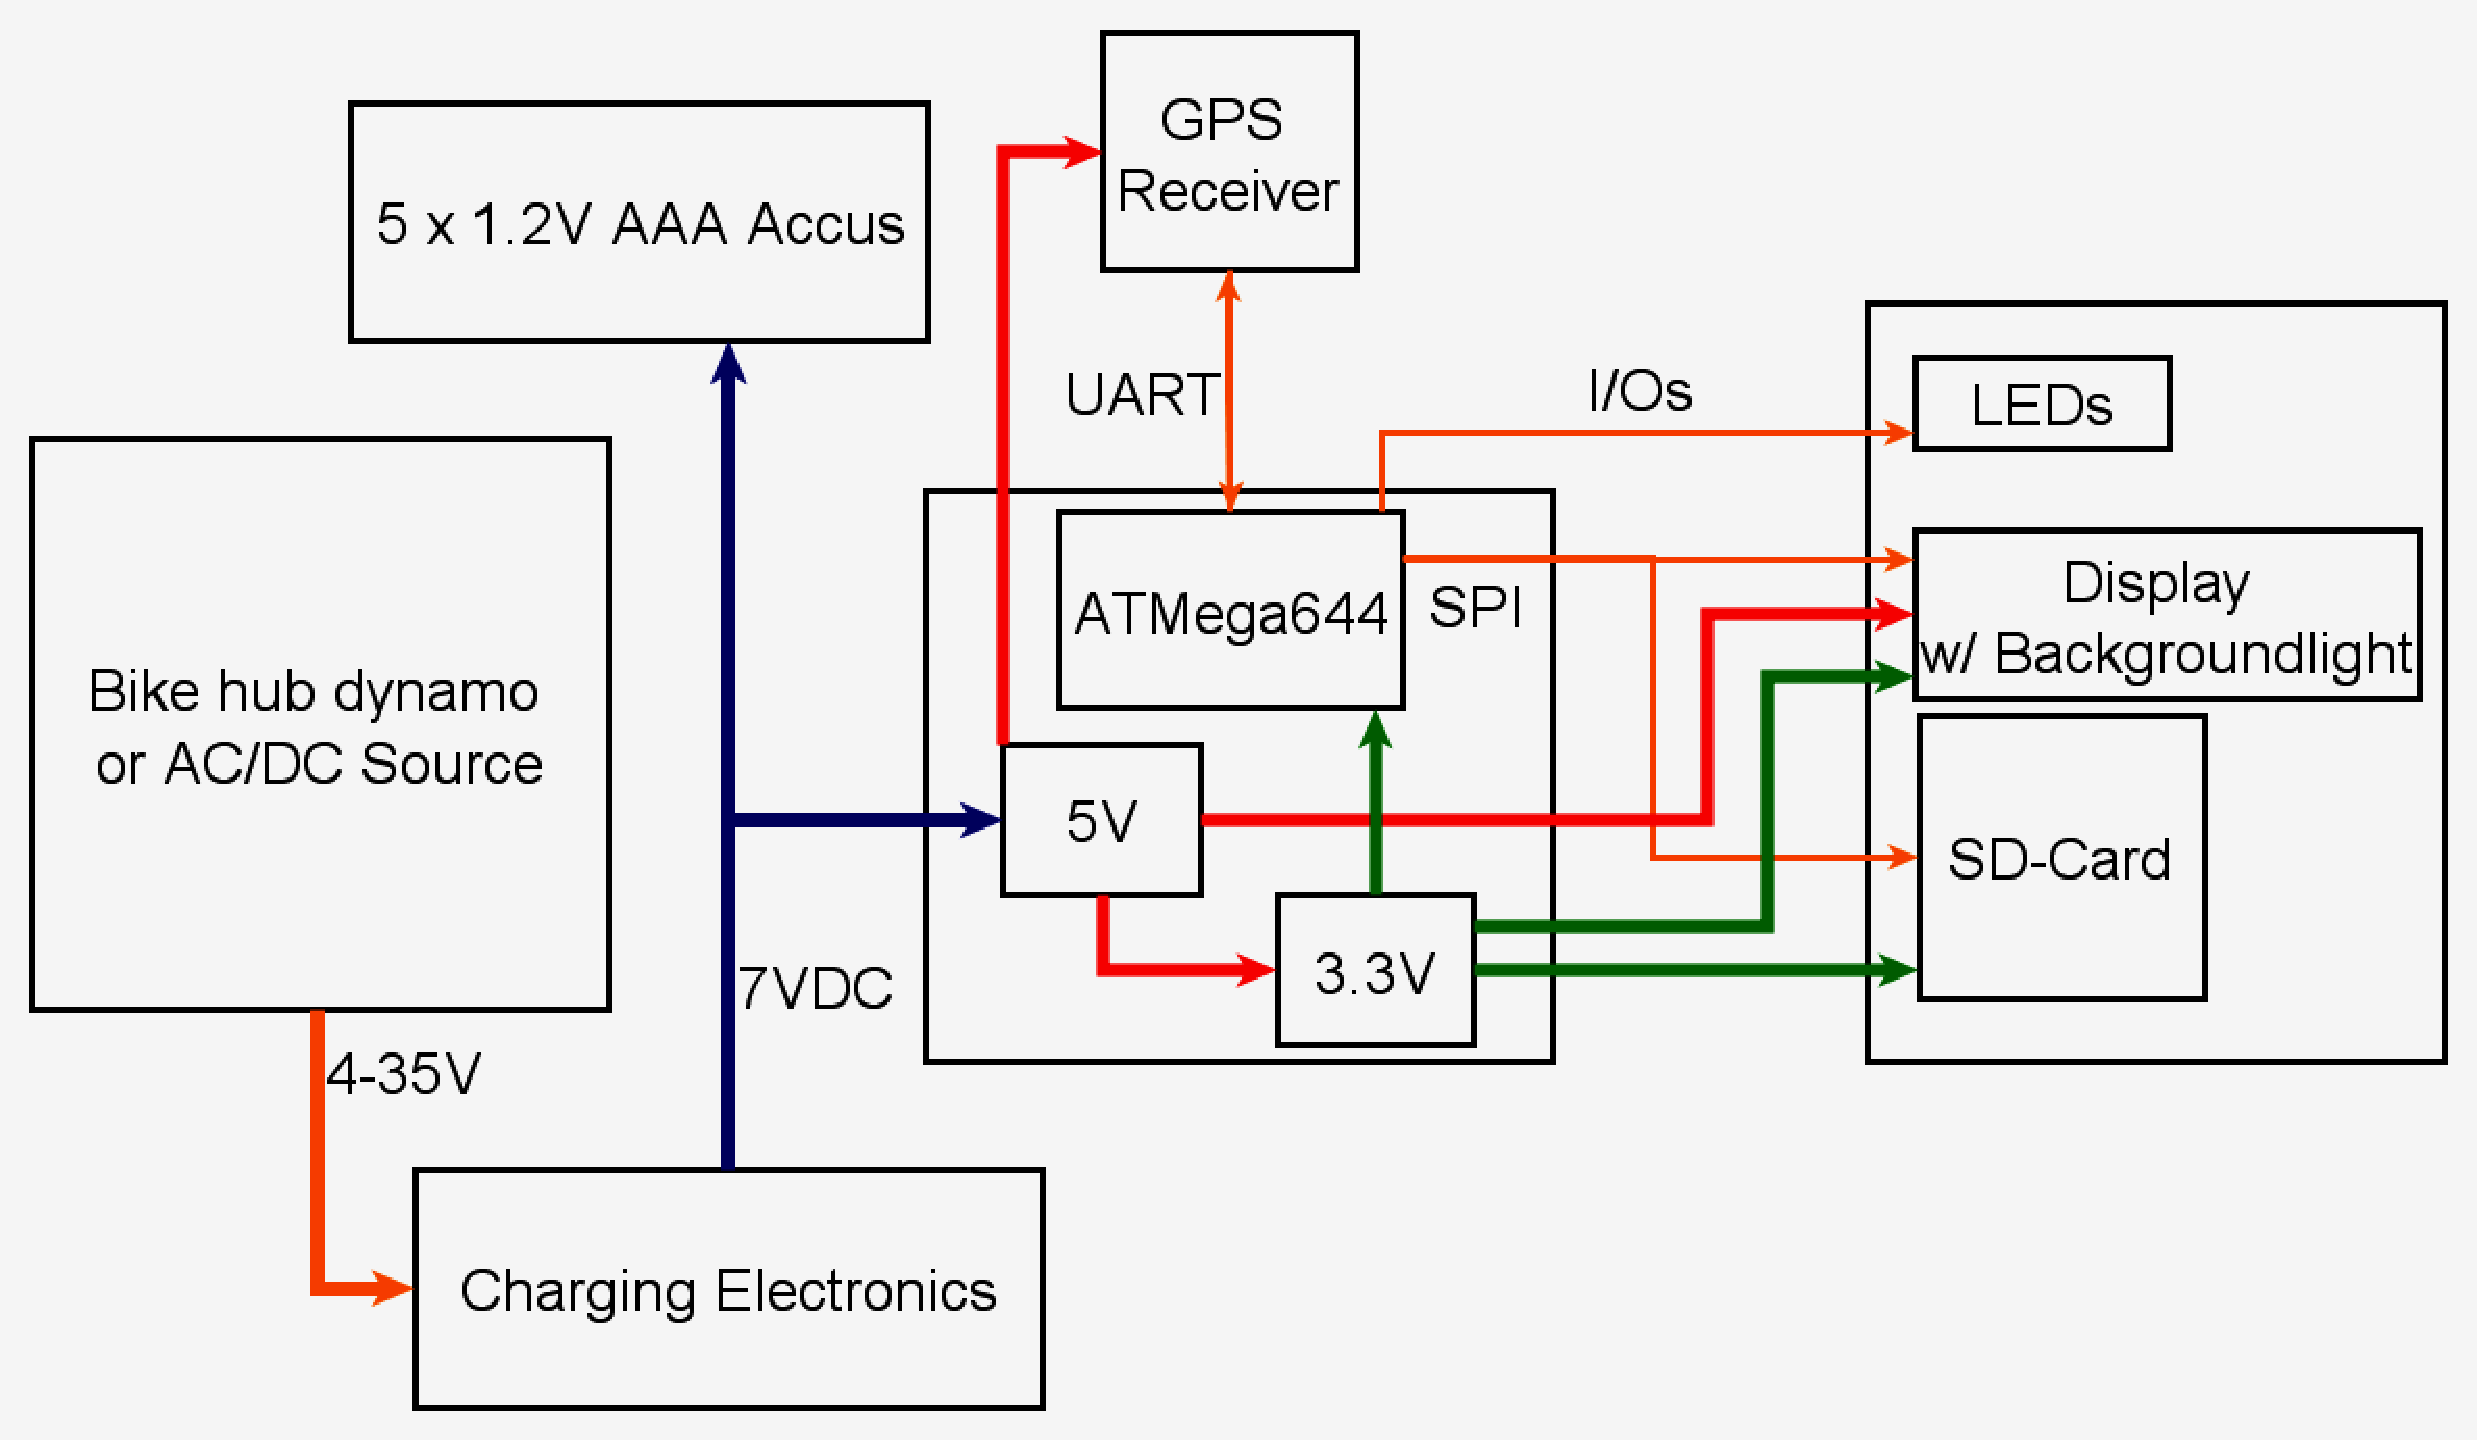
\includegraphics[width=\textwidth]{blockschaltbild}


\section{Software}
\subsection{Design topics}
\begin{itemize}
\item Mapping features to various modules - The functionality is separated to different modules (e.g. GPS module, Interrupt module, ...)
\item Running synchronous to GPS data receiving (triggered by USART interrupt)
\begin{itemize}
\item no timing/scheduling problems
\item simple integration of the basic features
\item no OS required
\item but: no complex user interaction possible (e.g. via touch screen)
\end{itemize}
\item no OS is used
\begin{itemize}
\item integration too time consuming
\item functions have to be reentrant
\item balancing of tasks pretty time consuming and complex (detailed design necessary)
\end{itemize}
\end{itemize}

\subsection{The NMEA/PUBX Protocol}
\begin{itemize}
\item NMEA: simple (serial) ASCII protocol (standardized)
\item PUBX: proprietary NMEA extension (used for configuration)
\end{itemize}

\subsection{Components}
\subsubsection{SPI (Serial Peripheral Interface)}
\begin{itemize}
\item simple SPI-driver
\item used for communication between $\mu$C and SD card and the display 
\end{itemize}

\subsubsection{Display}
\textbf{Setting single pixels}
\begin{figure}[hb]
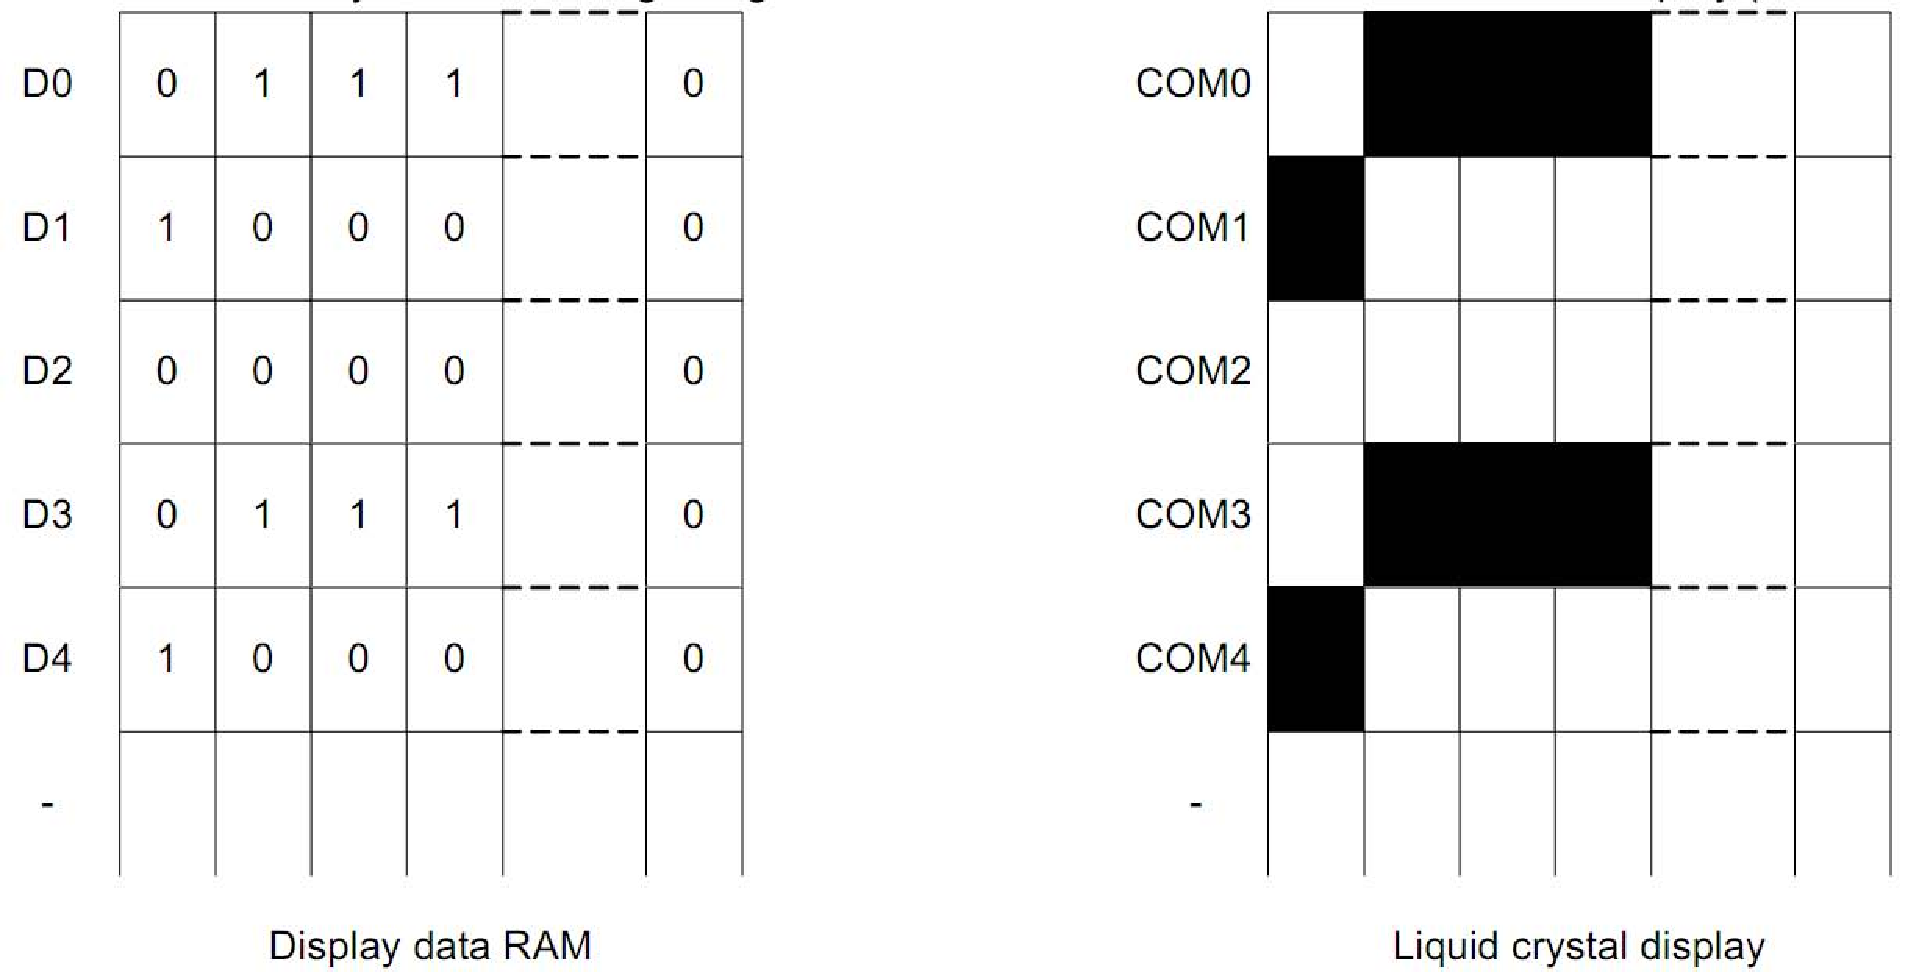
\includegraphics[width=\textwidth]{display_ram}
\end{figure}
\begin{itemize}
\item direct pixel access via display data RAM
\item RAM is organized in pages
\item total size of $(8 pages * 8 bit) * 132 bit$ (actual only 128 bit, because of the display resolution of 128 x 64)
\item internal SW buffer: sequential data structure (8 bit data type)
\item positioning within the internal buffer for setting a pixel with coordinates X and Y: $INDEX = (Y * 8) + (X / 8)$
\item the actual bit is determined by : $BIT\_NR = Y \& 0x07$ (determining the actual row within a memory page)
\item Summary: the index of the data buffer represents the 'column' number within the data memory (of a single page), the result of a bit-wise AND
operation with Y results in the actual row of the respective memory page
\end{itemize}
\begin{figure}[htb]
\lstinputlisting[language=C,label=put_pixel_function,caption=Example: display\_putpixel() function]{put_pixel.c}
\end{figure}

\textbf{Drawing BMPs/Text}
\begin{itemize}
\item BMPs: Converting BMPs into simple C-Arrays
\item Text: using a 5x7 character set (organized in a simple one dimensional array)
\end{itemize}

\subsubsection{LEDs}
\begin{itemize}
\item simple IO access
\item used as status indicator
\item e.g. receiving of GPS data, recording of GPS data, ...
\end{itemize}

\subsubsection{UART (Universal Asynchronous Receiver Transmitter)}
\begin{itemize}
\item simple driver module
\item used for communication between PC and $\mu$C
\item or between GPS and $\mu$C
\end{itemize}

\subsubsection{GPS}
\begin{itemize}
\item initialization of the GPS receiver:
\begin{itemize}
\item setting the baud rate (for synchronization with the $\mu$C
\item setting refresh rate to 1 per second (supports also 4)
\item selection of required data sets (RMC, GGA, VTG)
\end{itemize}
\item splitting of NMEA data sets (',*' separator)
\item storage into internal data structure
\end{itemize}

\subsubsection{SDC/FAT16}
\begin{itemize}
\item tiny open source library
\item horrible code (e.g. huge amount of magic numbers, magic bit shifting with several side effects)
\end{itemize}

\subsubsection{Touch screen}
\begin{itemize}
\item used for start/stop data recording
\item connected to MC via ADC
\end{itemize}

\section{References}
\begin{itemize}
\item http://www.lcd-module.de/pdf/grafik/dogl128-6.pdf, Electronic Assembly
\item NL\_u-blox5\_Referenzmanual\_06102008\_571.pdf, u-blox 5 NMEA, UBX Protocol Specification
\item http://www.atmel.com/dyn/resources/prod\_documents/doc2593.pdf, ATmega644L datasheet
\item http://focus.ti.com/lit/ds/symlink/max3221.pdf, MAX3221 datasheet
\item http://www.national.com/ds/LM/LM3478.pdf, LM3478 Switching Regulator datasheet
\item http://www.lcd-module.de/eng/pdf/zubehoer/st7565r.pdf, ST75565R display controller data sheet
\end{itemize}

\end{document}